\documentclass{article}

% Language setting
% Replace `english' with e.g. `spanish' to change the document language
\usepackage[spanish]{babel}

% Set page size and margins
% Replace `letterpaper' with `a4paper' for UK/EU standard size
\usepackage[letterpaper,top=2cm,bottom=2cm,left=3cm,right=3cm,marginparwidth=1.75cm]{geometry}

% Useful packages
\usepackage{amsmath}
\usepackage{graphicx}
\usepackage[colorlinks=true, allcolors=blue]{hyperref}

\title{Resolución práctica 13}
\author{Marcelo Antony Pérez Treviños}

\begin{document}
\maketitle
\section{Fish class en javascript}

Se dice que un lenguaje de programación tiene características de primera clase si las características se tratan como cualquier otra variable en ese lenguaje. Por ejemplo, el lenguaje permite pasar funciones como argumentos a otras funciones, devolverlas desde otras funciones y asignarlas a variables. El siguiente ejemplo muestra la importancia de conocer las características de primer nivel.

\subsection{Ejemplo:}

\begin{verbatim}

// first class functions

function Person(name, lastname)
{
    this.name = name || 'Maruchan';
    this.lastname = lastname || 'Espiritusanto';
    
    this.greet = function ()
    {
        return 'Hello '+ this.name + ' your lastname is '+ this.lastname;
    }
}

var mario = new Person('Mario', 'Castillo');
var daniel = new Person();

//console.log(mario);
//console.log(daniel.greet());

function executeFunctionPerson (person)
{
    console.log(person.greet()); // Hello Mario your lastname is Castillo
}
executeFunctionPerson(mario);

\end{verbatim}

\begin{figure}
\centering
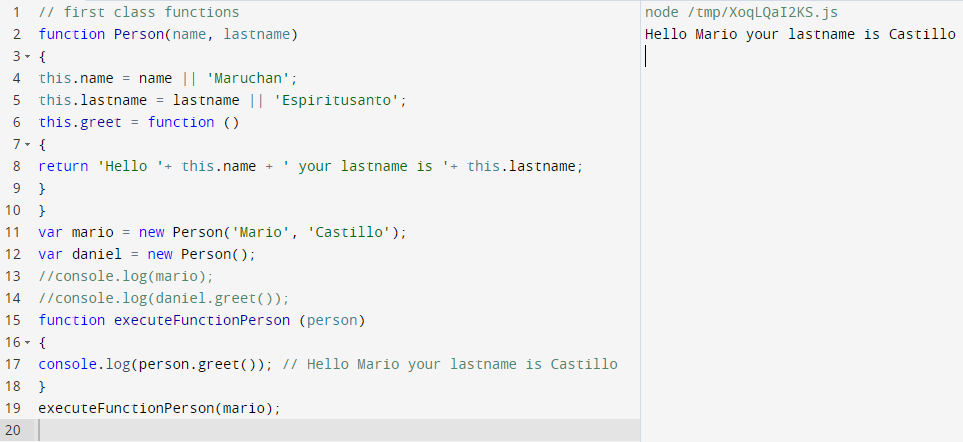
\includegraphics[width=1\textwidth]{ejercicio1.png} 
\caption{\label{fig:frog}Código y ejecución del ejercicio 1}
\end{figure}

\section{Diferencia entre Currying and Partial Application}

La forma más fácil de ver en qué se diferencian es ver un ejemplo de trabajo. Suponga que tiene una función Agregar que toma dos números como entrada y devuelve un número como salida. B. Sumar(7, 5) devuelve 12, en este caso:

\subsection{Partial Application}

la función Add con un valor 7 nos dará una nueva función como salida. Esa función en sí toma 1 número como entrada y genera un número. Como tal:

\begin{verbatim}
Partial(Add, 7); // devuelve una función f2 como salida

                 // f2 toma 1 número como entrada y devuelve un número como salida
\end{verbatim}
Entonces podemos hacer esto:

\begin{verbatim}
f2 = Partial(Add, 7);
f2(5); // devuelve 12;
       // f2(7)(5) es solo un atajo sintáctico
\end{verbatim}

\subsection{Currying}

la función Addnos dará una nueva función como salida. Esa función en sí toma 1 número como entrada y genera otra función nueva. Esa tercera función luego toma 1 número como entrada y devuelve un número como salida. Como tal:

\begin{verbatim}
Curry(Add);  // devuelve una función f2 como salida

             // f2 toma 1 número como entrada y devuelve una función f3 como salida
             // es decir, f2(número) = f3

             // f3 toma 1 número como entrada y devuelve un número como salida
             // es decir, f3(número) = número
\end{verbatim}

Entonces podemos hacer esto:

\begin{verbatim}
f2 = Curry(Add);
f3 = f2(7);
f3(5); // devuelve 12
\end{verbatim}

En otras palabras, currying y partial Application son  funciones completamente diferentes. Currying requiere exactamente una entrada, mientras que partial Application requiere dos o más entradas. Como puede ver arriba, ambas funciones devuelven como salidas, pero las funciones devueltas se devuelven de formas completamente diferentes.

\section{Implemente una función que calcule el volumen de un cilindro. Incluya la versión normal y una aplicando Currying.}

\begin{verbatim}
function volume(altura, diametro) {
    
    return (altura * Math.PI * (diametro/2)).toFixed(4);
}

function curriedVolume(altura) {
    return function(diametro) {
        return (altura * Math.PI * (diametro/2)).toFixed(4);
    }
}

console.log(volume(5, 2)); // 15.7080
console.log(curriedVolume(5)(2)); // 15.7080
\end{verbatim}

\begin{figure}
\centering
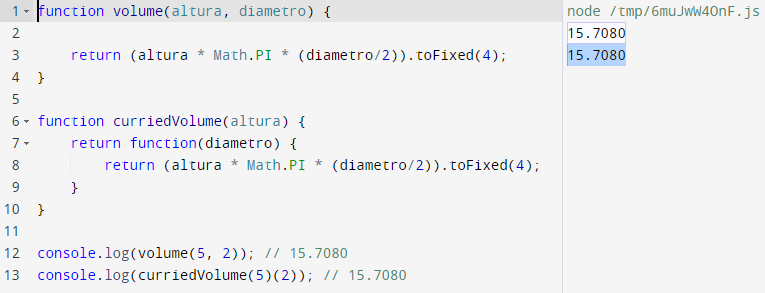
\includegraphics[width=1\textwidth]{ejercicio3.png}
\caption{\label{fig:frog}Código y ejecución del ejercicio 3}
\end{figure}

\section{Cree una función joinWords que una varios parametros de tipo string}

\begin{verbatim}
function joinWords(w1) {
  return function (w2) {
    if (w2 == null) {
      return `${w1}`;
    } else {
      return function (w3) {
        if (w3 == null) {
          return `${w1}${w2}`;
        } else {
          return function (w4) {
            if (w4 == null) {
              return `${w1}${w2}${w3}`;
            } else {
              return function (w5) {
                if (w5 == null) {
                  return `${w1}${w2}${w3}${w4}`;
                }
              }
            }
          };
        }
      };
    }
  };
}

result = joinWords('Hello ')();
console.log(result); // Hello

result = joinWords ('There ')('is ')('no ')('spoon .')();
console.log(result); // There is no spoon .
\end{verbatim}

\begin{figure}
\centering
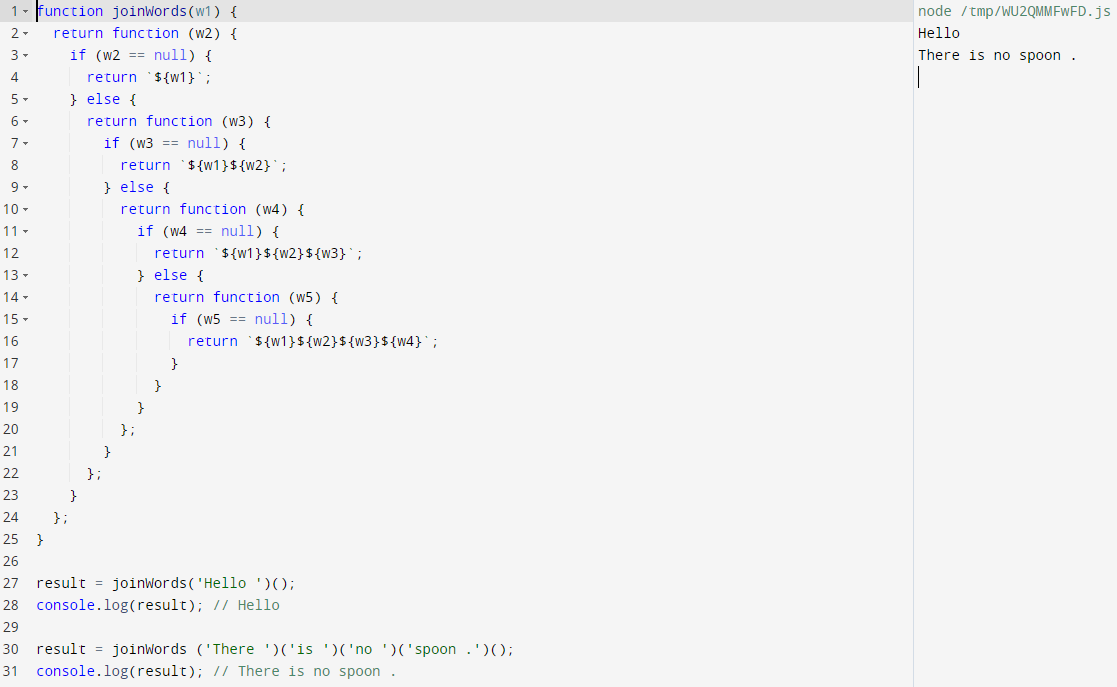
\includegraphics[width=1\textwidth]{ejercicio4.png}
\caption{\label{fig:frog}Código y ejecución del ejercicio 4}
\end{figure}

\section{Implemente una función  delayInvoc que en cada invocaci ́on incremente la variable total con el valor enviado como parámetro.}

\begin{verbatim}
var total = 0;
var delayInvoc = function (a) {
  return function (b) {
    total = a + b;
    return function (c) {
      return (total = total + a + b + c);
    };
  };
};
delayInvoc(4)(5);
console.log(total); //9
delayInvoc(4)(5)(8);
console.log(total); // 26
\end{verbatim}

\begin{figure}
\centering
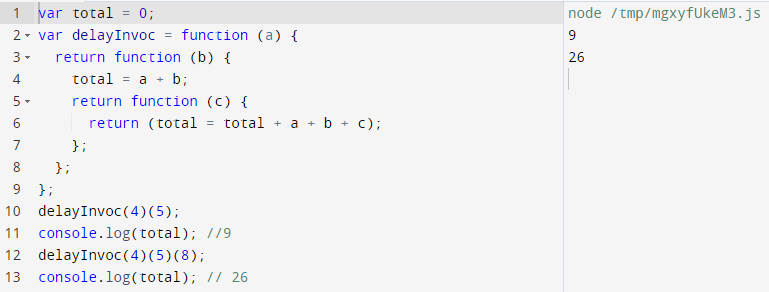
\includegraphics[width=1\textwidth]{ejercicio5.png}
\caption{\label{fig:frog}Código y ejecución del ejercicio 5}
\end{figure}

\section{Implemente una función curry que tome como argumento cualquier función f y retorne la versión curried de f.}

\begin{verbatim}
function abc(a, b, c) {
  return a + b + c;
}
function curry(f) {
  return function curried(...argum) {
    if (argum.length >= f.length) {
      return f.apply(this, argum);
    } else {
      return function (...args2) {
        return curried.apply(this, argum.concat(args2));
      };
    }
  };
}
var curriedAbc = curry(abc);
console.log(curriedAbc(2)(3)(4)); // 9
console.log(curriedAbc(2, 3)(4)); // 9
console.log(curriedAbc(2)(3, 4)); // 9
console.log(curriedAbc(2, 3, 4)); // 9
\end{verbatim}

\begin{figure}
\centering
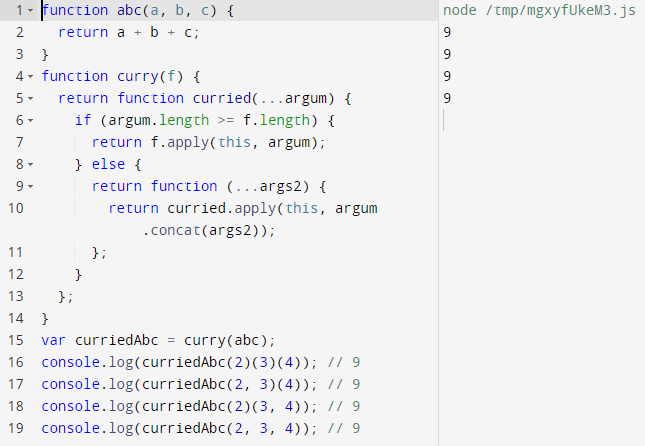
\includegraphics[width=1\textwidth]{ejercicio6.png} 
\caption{\label{fig:frog}Código y ejecución del ejercicio 6}
\end{figure}

\end{document}